\section{Principali scadenze e procedure da attivare}
\subsection{Procedura laurea}
Al seguente link potrai trovare una guida sulle principali scadenze e procedure da attivare:
https://web.unisa.it/didattica/segreteria/servizi?servizio=20 \\
\underline {Sii tu a ricordarle alla persona che ti segue!}
\subsection{Esame di Tirocinio}

Al seguente link trovi il registro da compilare: https://corsi.unisa.it/05121/modulistica 

\noindent Per le attività da inserire sii generico, puoi mettere anche per più giorni, ad esempio: ricerca bibliografica, studio di Python, studio di tecniche di ML, studio del dataset, implementazione, analisi dei risultati ecc. Attenzione ai giorni festivi o a quelli dove ad esempio si è impegnati con gli esami,  \textbf{non} vanno inseriti. Inoltre, sarebbe opportuno non eccedere le 6 ore giornaliere. \underline {Sii tu a ricordarlo alla persona che ti segue!}

\subsubsection{Quante ore?}
\begin{itemize}
    \item \textbf{STUDENTE TRIENNALE}\\
    Al seguente link puoi trovare le informazioni che cerchi:\\
https://corsi.unisa.it/informatica/didattica/insegnamenti

\item \textbf{STUDENTE MAGISTRALE}\\
    Al seguente link puoi trovare le informazioni che cerchi:\\
https://corsi.unisa.it/informatica-magistrale/didattica/insegnamenti

\end{itemize}

\section{Lavoro Svolto}
Tutto ciò che produci deve essere condiviso con la persona che ti segue. Il codice è il caso di condividerlo con un file \textbf{jupyter} opportunamente commentato in ogni sua parte dove si stampano gli output di tutto ciò che è possibile mostrare per renderne più immediata la comprensione. 



\section{Come si organizza una tesi?}
In generale la struttura di una tesi è così articolata:
\begin{itemize}
    \item \textbf{Abstract:} è una descrizione \textit{sintetica} di tutto il lavoro che nello spazio di una pagina o anche meno riassume:
    \begin{enumerate}
        \item il campo applicativo della tesi
        \item il problema affrontato
        \item il metodo di sperimentazione proposto
        \item brevi evidenze dei risultati ottenuti
        \item conclusioni
    \end{enumerate}
    Lo spirito con cui si scrive l'abstract è quello secondo cui un lettore può leggerlo e farsi immediatamente una idea del suo contenuto
 \item \textbf{Capitolo 1}: introduzione al problema
 \item \textbf{Capitolo 2}: inquadramento del problema, con eventuale riferimento a lavori simili in letteratura, e i suoi campi applicativi
 \item \textbf{Capitolo 3}: la fase vera del lavoro di tesi con la spiegazione teorica delle varie tecniche utilizzate
 \item \textbf{Capitolo 4}: risultati raggiunti e sperimentazione. Descrizione del codice nelle sue parti salienti  
 \item \textbf{Conclusioni e possibili sviluppi futuri}
\end{itemize}

\subsection{Tabelle}
Per creare le tabelle ti consiglio: https://www.tablesgenerator.com/

\subsection{Bibliografia}
Ecco una dimostrazione di come fare una citazione: \cite{introduction_biometric}.  Ricorda che ci sono gli hyperlink, quindi prova a cliccare sulla citazione sul documento compilato. \\


\subsubsection{Dove fare le ricerche?}
Ti consiglio di fare le ricerche su Google Scholar e Scopus (https://www.scopus.com/standard/marketing.uri). Per quest'ultimo probabilmente dovrai prima cambiare le impostazione del proxy. Al seguente link ti viene spiegato come fare:\\ https://www.unisa.it/uploads/852/manuale\_configurazione\_proxy2019.pdf 

\noindent Per quanto riguarda la questione degli articoli a pagamento puoi utilizzare il seguente link (la legalità del sito è, diciamo, controversa):
      https://scihub.bban.top
Ti basterà inserire il DOI dell'articolo a cui sei interessato. Il DOI è un codice che identifica univocamente un articolo, se ad esempio usi SCOPUS lo puoi trovare in basso a destra, come nell'immagine \ref{fig:esempio}:

\begin{figure}[ht!]
    \centering
    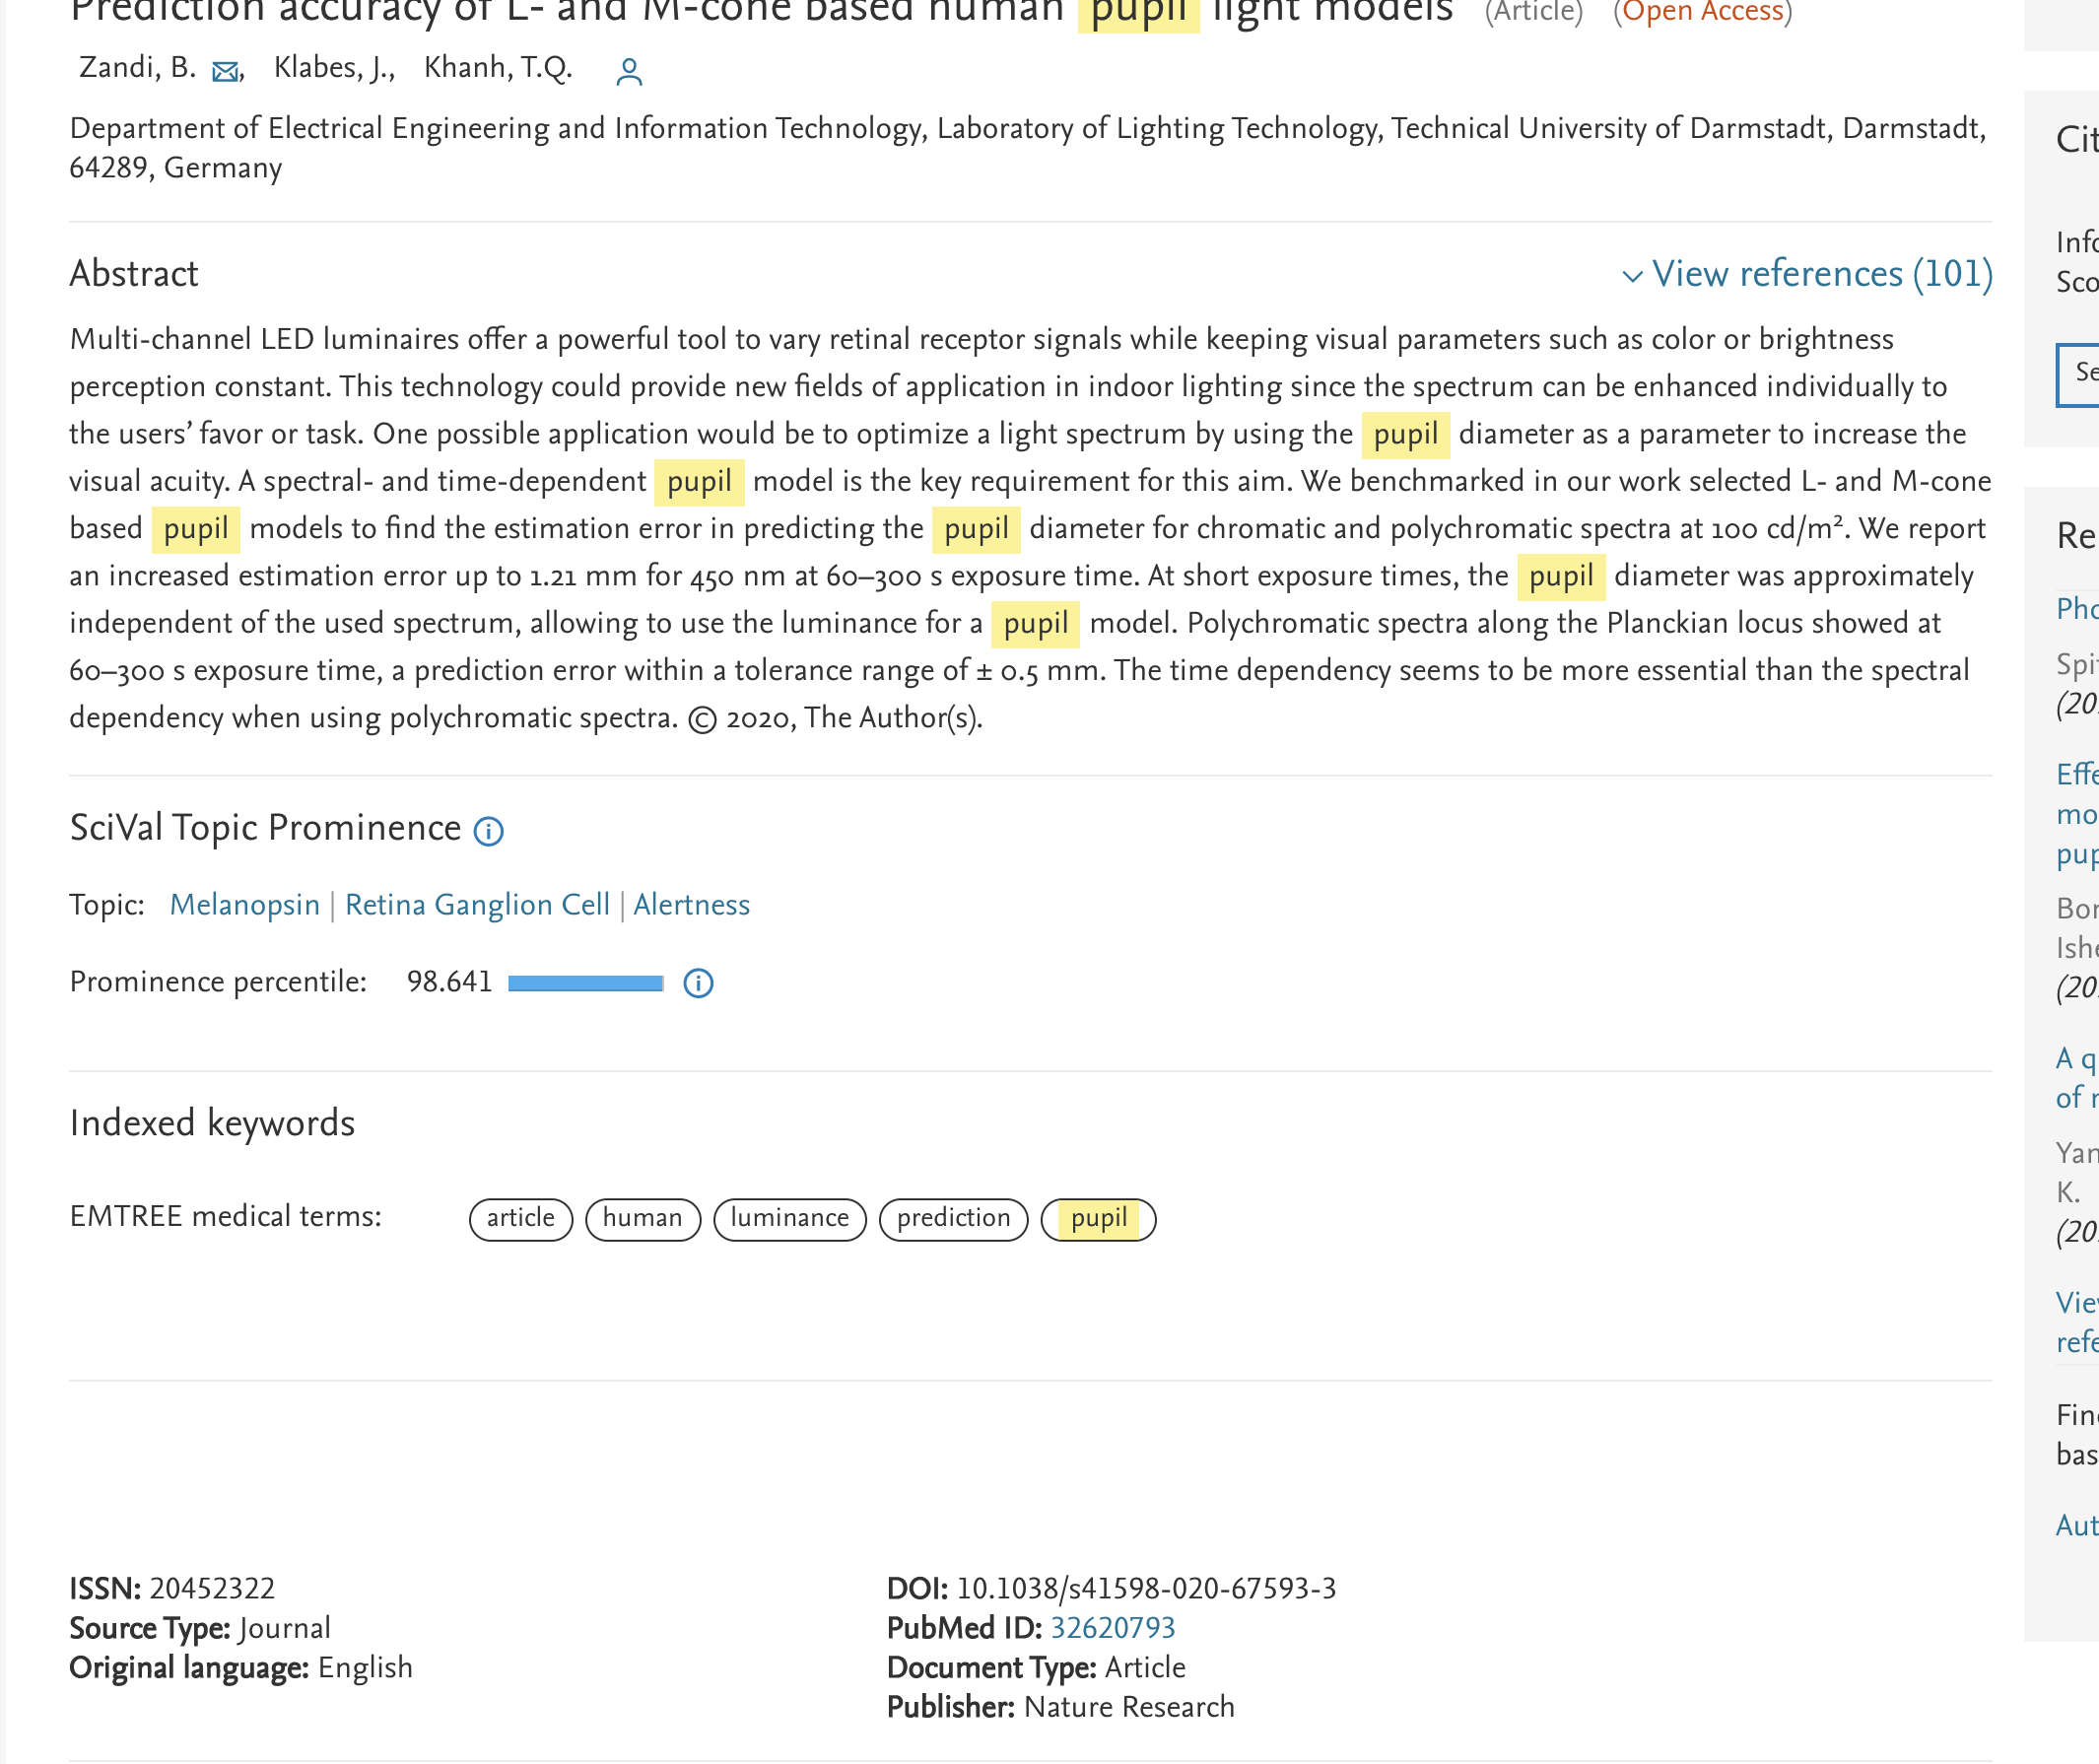
\includegraphics[width=4in]{Figure/Schermata 2020-07-22 alle 13.59.57.png}
    \caption{Esempio}
    \label{fig:esempio}
\end{figure}



\noindent Ti basterà quindi copiare la dicitura "DOI: 10 ..." nella barra di ricerca che trovi al link che ti ho suggerito e il gioco è fatto.


\subsubsection{Come citare gli articoli?}
Il modo più semplice per aggiungere articolari da citare al file `bibliografia.bib' è
\begin{itemize}
    \item su Google Scholar: cercare l'articolo che ti interessa, cliccare sul simbolo ` " ' ed infine selezionare BibTex e fare copia-incolla 
    
    \item su SCOPUS: dopo aver cliccato sul lavoro, nella pagina in cui compare l'abstract come in Figura \ref{fig:esempio}, in alto a sinistra trovi ``BibTex export''
\end{itemize}

\subsection{Suggerimenti ed Errori comuni da NON fare}
\begin{itemize}
    \item Le figure vanno accompagnate sempre da una label, vanno numerate e richiamate nel testo
    \item Le formule vanno numerate
    \item Standardizza l'uso delle maiuscole: se decidi di usare la lettera maiuscola per una certa parola poi continua così per l'intero documento
    \item Attento alle virgolette ``aperte''. Vedi in questo sorgente come vanno messe. Se hai un Mac ti basta fare ``\textit{option+9}''
    \item In riferimento al codice,  questo deve far parte del testo principale della tesi quando si presenta qualche implementazione originale o qualche algoritmo proposto dallo stesso tesista. Quando si tratta di codice di routine che implementa concetti noti, la collocazione più appropriata sarebbe in una sezione dedicata e rinominata come \textit{Appendice } (che si trova sempre infondo alla tesi) https://tesinsieme.it/appendici-della-tesi-di-laurea-guida-definitiva-in-4-punti/

\end{itemize}

\subsection{Correzioni}

Le correzioni all'elaborato verranno apportate direttamente sul sorgente dell'Overleaf condiviso attraverso i ``commenti''. \textbf{Non} ``risolverli'' tu, sarà la persona che ti segue a farlo una volta appurato che le modifiche/integrazioni vadano bene.

\section{Ultimo sforzo... la presentazione}
Nella progettazione di una presentazione per un lavoro (che si parli di una tesi o di qualsivoglia presentazione di un elaborato), il mio consiglio è quello di "buttare" nella presentazione una grossa quantità di informazioni e poi lavorare per sottrazione. Scremando ed eliminando argomenti/slide la presentazione prenderà man mano forma e sarà essa stessa a suggerirti qualche volta come andare avanti tra un discorso e l'altro. L'idea di base è di rendere chiari nel tuo discorso tre punti:
\begin{itemize}
    \item Obiettivo
    \item Approccio
    \item Risultati
\end{itemize}
